\documentclass{xjtureport}
\usepackage{graphicx}
\usepackage{float}
% =============================================
% Part 0 Edit the info
% =============================================

\major{大数据管理与应用}
\name{郅啸淇}
\title{最优化第四次作业}
\stuid{2184114639}
\college{管理学院}
\date{\zhtoday}
\lab{寝室}
\course{最优化理论与算法II}
\instructor{Xiangyu Chang}
\grades{??}
\expname{第四次作业题}
\exptype{完成作业}
\partner{Nobody}

\begin{document}
% =============================================
% Part 1 Header
% =============================================
\makecover

\makeheader

% =============================================
% Part 2 Main document
% =============================================

\section{HW1}
LASSO Problem
$x^* = \mathop{argmin}_{x} \{ \frac{1}{2} \| A\textbf{x} - b \| ^2 + \lambda \| \textbf{x} \|_{1}\}$

定义
$f^{t}_{k}(x_{k}) = f(x^{t+1}_{<k},x_{k},x^{t}_{>k})$

原LASSO问题等价于
$\mathop{\min}_{x} \{\frac{1}{2} \|b_i - \sum_{i =1}^{n} x_iA_i \| ^2+ \lambda \sum_{i=1}^{n}x_i\}$

其中$A = [A_1,A_2,...,A_n], b_i = b - \sum_{j \neq i} x_jA_j$

当$i = 1$,$x_2,...x_n$固定时

原式为$\mathop{\min}_{x} \{ \frac{1}{2} \|b_1 -  x_1A_1 \|^2 + \lambda  x_1 \}$

令$g(x) =\frac{1}{2} \|b_1 -  x_1A_1 \|^2 + \lambda x_1 $\

当$x_1 > 0$时,$\nabla_x g(x) = -A_1(b_1 - x_1A_1) + \lambda = 0$

$x_1 = (A^TA)^{-1}(A_1b_1 - \lambda)$

当$x_1 < 0$时,$x_1 = (A^TA)^{-1}(A_1b_1 + \lambda)$

当$x_1 = 0$时,$0 \in -A^T_1(b_1 - x_1A_1) + \lambda \partial |0|$

故
$x_i = \left\{\begin{matrix}
    (A^TA)^{-1}(A_nb_n - \lambda)  & x_i > 0\\ 
    (A^TA)^{-1}(A_nb_n + \lambda)&  x_i < 0 \\ 
    0&|A_i^Tb_i^T| \leq \lambda 
   \end{matrix}\right.$
\section{HW2}
Fused LASSO

$\mathop{\min}_{x}\{ \frac{1}{2} \|Ax - b  \|^2 + \lambda \|Bx\|\}$

等价于
\begin{equation}
    \begin{aligned} \label{P}
        & \mathop{\min}_{x}\{ \frac{1}{2} \|Ax - b  \|^2 + \lambda \|z\|\}\\
        &\begin{array}[]{r@{\quad}r@{}l@{\quad}l}
        s.t.& Bx - z = 0\\
        \end{array}
    \end{aligned}
\end{equation}

增广Lagrange函数为$L_{\rho}(x,z,v) = \frac{1}{2} \|Ax - b \| ^2 + \lambda \|z\| + v^T(Bx-z) + \frac{\rho}{2} \|Bx-z\|^2$

$\left\{\begin{matrix}
    x^{t+1} =\mathop{argmin}_{x}L_\rho (x,z^t,v^t)\\ 
    z^{t+1} =\mathop{argmin}_{x}L_\rho (x^{t+1},z,v^{t})\\ 
    v^{t+1} = v^t + \rho(Bx^{t+1} -z^{t+1}) 
   \end{matrix}\right.$

令$u = \frac{v}{\rho}$

$x^{t+1} = \mathop{argmin}_{x} \{\frac{1}{2} \| Ax - b\|^2 + \frac{\rho}{2} \| Bx - z^t +u^t\|^2\}$

令$g(x) = \frac{1}{2} \| Ax - b\|^2 + \frac{\rho}{2} \| Bx - z^t +u^t\|^2$

$\nabla g(x) = A^T(Ax -b) + \rho(x-z^t+u^t) = 0$

$x^{t+1} = (A^TA+\rho I)^{-1}(A^Tb + \rho z^t - \rho u^t)$

$z^{t+1} = \mathop{argmin}_{x} \{\lambda \|z\| + \frac{\rho}{2} \|Bx^{t+1} + u^t - z\|^2\}$

$\Rightarrow \mathop{prox}_{\frac{\lambda}{\rho} \|z\|}(Bx^{t+1} + u^t)$

$=sign(Bx^{t+1} + u^t)(|Bx^{t+1} + u^t| - \frac{\lambda }{\rho})_+$

$u^{t+1} = u^t + Bx^{t+1} -z^{t+1}$

$\left\{\begin{matrix}
    x^{t+1} =(A^TA+\rho I)^{-1}(A^Tb + \rho z^t - \rho u^t)\\ 
    z^{t+1} =sign(Bx^{t+1} + u^t)(|Bx^{t+1} + u^t| - \frac{\lambda }{\rho})_+\\ 
    u^{t+1} = u^t + Bx^{t+1} -z^{t+1} 
   \end{matrix}\right.$
\section{HW3}
原问题
\begin{equation}
    \begin{aligned} \label{P}
        & \mathop{\min}_{x}\{ \|x\|_1\}\\
        &\begin{array}[]{r@{\quad}r@{}l@{\quad}l}
        s.t.& Ax = b\\
        \end{array}
    \end{aligned}
\end{equation}

等价于
\begin{equation}
    \begin{aligned} \label{P}
        & \mathop{\min}_{x}\{ \|z\| + f(x)\}\\
        &\begin{array}[]{r@{\quad}r@{}l@{\quad}l}
        s.t.& x - z = 0\\
        \end{array}
    \end{aligned}
\end{equation}

其中$f(x)=\left\{\begin{matrix}
    0,if Ax = b\\ 
    +\infty,if Ax \neq b  
   \end{matrix}\right.$

$L_\rho (x,z,v) = \left\{\begin{matrix}
    \|z\| + v^T(x-z) + \frac{\rho}{2} \|x-z \|^2\\ 
    +\infty,if Ax \neq b
   \end{matrix}\right.$

$ \left\{\begin{matrix}
x^{t+1} =\mathop{argmin}_{x}L_\rho (x,z^t,v^t)\\ 
z^{t+1} =\mathop{argmin}_{x}L_\rho (x^{t+1},z,v^{t})\\ 
v^{t+1} = v^t + \rho(Bx^{t+1} -z^{t+1}) 
\end{matrix}\right.$

$x^{t+1} = \mathop{argmin}_x \{v^T(x-z^t) + \frac{\rho}{2}\|x -z^t\|^2\}$

$= \mathop{argmin}_x\{ \frac{\rho}{2}\|x -z^t + u^t\|^2\}$

$ = \pi_\omega(z^t - u^t)$

其中$\omega = \{ x| Ax  = b \} $

由上次作业结论$x^{t+1} = (z^t - u^t) - A^T(A^TA)^{-1}[A(z^t-u^t)-b]$

$z^{t+1} = \mathop{argmin}_{x} \{ \|z\| + \frac{\rho}{2} \|x^{t+1} + u^t - z^t\|^2\}$

$= \mathop{prox}_{\frac{\|z\|}{\rho}}\{ x^{t+1} - u^t\}$

$= sign(x^{t+1} - u^t)(|x^{t+1} - u^t| - \frac{1}{\rho})_+$

$u^{t+1} = u^t + x^{t+1} -z^{t+1}$


$\left\{\begin{matrix}
    x^{t+1} =(z^t - u^t) - A^T(A^TA)^{-1}[A(z^t-u^t)-b]\\ 
    z^{t+1} =sign(x^{t+1} - u^t)(|x^{t+1} - u^t| - \frac{1}{\rho})_+\\ 
    u^{t+1} = u^t + x^{t+1} -z^{t+1} 
   \end{matrix}\right.$
\section{HW4}
\lstinputlisting[language=Python]{LASSO_Proximal_BCD_ADMM.py}
\subsection{Proximal Gradient Descent}
$\lambda = 10$时,迭代结果为:$152.23667337896808$
\begin{figure}[H]
    \centering
    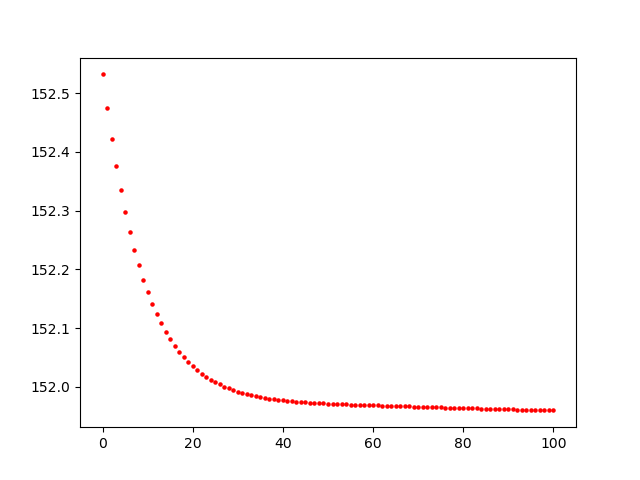
\includegraphics[scale = 0.6]{figures/Prox_lam=10.png}
    \caption{lambda = 10}
    \end{figure}
$\lambda = 1$时,迭代结果为:$17.47128983481235$
\begin{figure}[H]
    \centering
    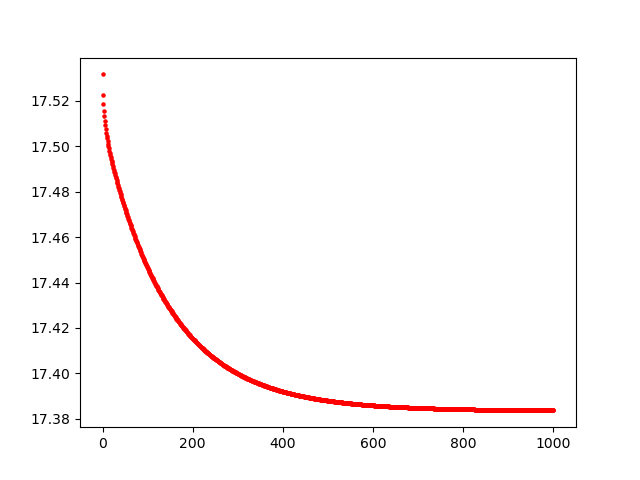
\includegraphics[scale = 0.6]{figures/Prox_lam=1.png}
    \caption{lambda = 1}
    \end{figure}
$\lambda = 0.1$时,迭代结果为:$3.587676594826708$
\begin{figure}[H]
    \centering
    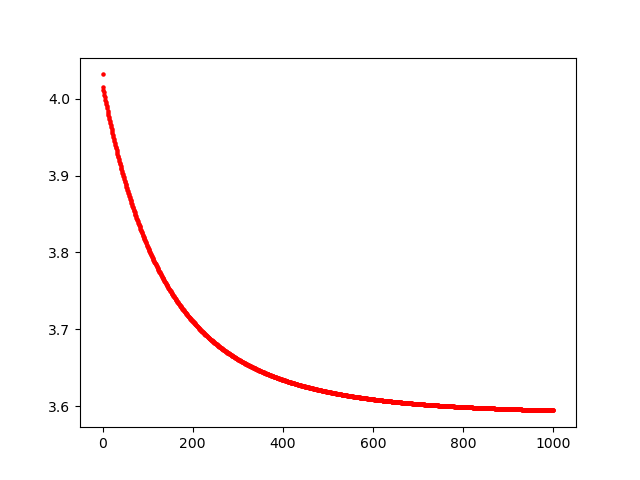
\includegraphics[scale = 0.6]{figures/Prox_lam=0.1.png}
    \caption{lambda = 0.1}
    \end{figure}
\subsection{BCD}
$\lambda = 10$时,迭代结果为:$152.23046561943306$
\begin{figure}[H]
    \centering
    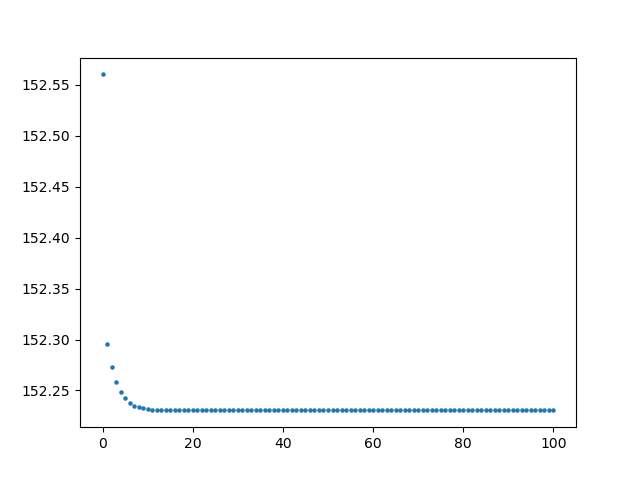
\includegraphics[scale = 0.6]{figures/BCD_lam=10.png}
    \caption{lambda = 10}
    \end{figure}
$\lambda = 1$时,迭代结果为:$17.5370839635338$
\begin{figure}[H]
    \centering
    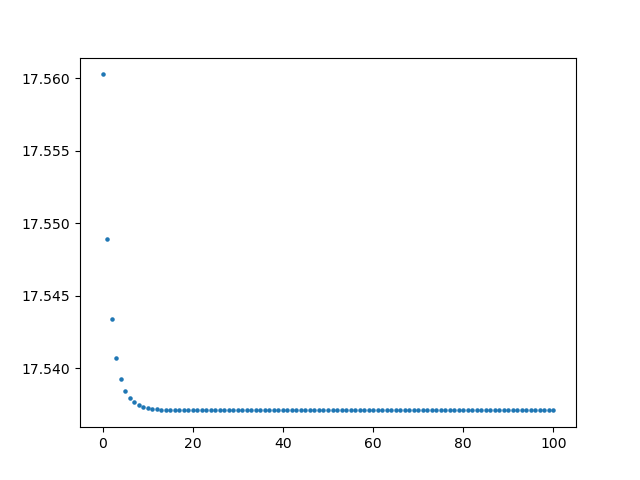
\includegraphics[scale = 0.6]{figures/BCD_lam=1.png}
    \caption{lambda = 1}
    \end{figure}
$\lambda = 0.1$时,迭代结果为:$4.0347736846143825$
\begin{figure}[H]
    \centering
    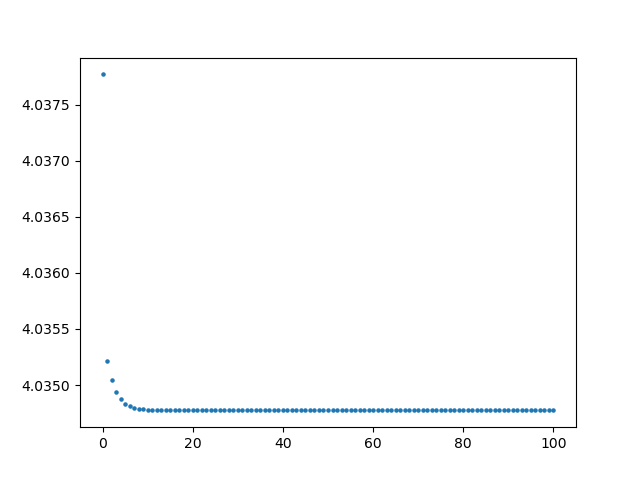
\includegraphics[scale = 0.6]{figures/BCD_lam=0.1.png}
    \caption{lambda = 0.1}
    \end{figure}
\subsection{ADMM}
$\lambda = 10$时,迭代结果为:$152.2382124270402$
\begin{figure}[H]
    \centering
    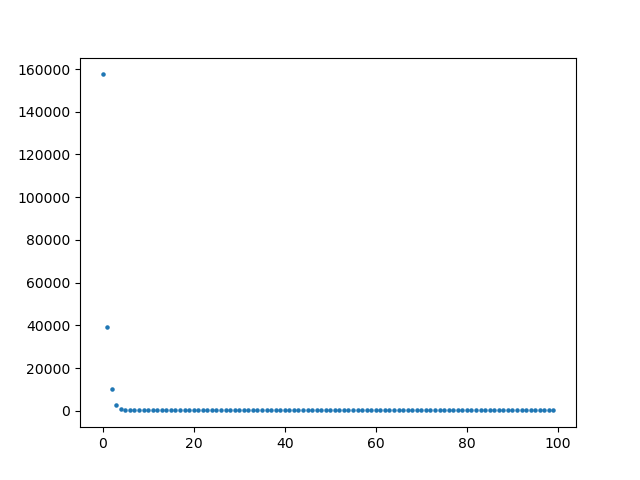
\includegraphics[scale = 0.6]{figures/ADMM_lam=10.png}
    \caption{lambda = 10}
    \end{figure}
$\lambda = 1$时,迭代结果为:$17.51542818309732$
\begin{figure}[H]
    \centering
    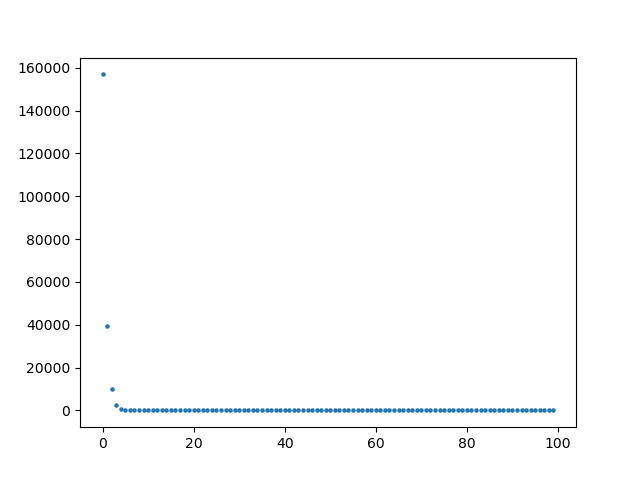
\includegraphics[scale = 0.6]{figures/ADMM_lam=1.png}
    \caption{lambda = 1}
    \end{figure}
$\lambda = 0.1$时,迭代结果为:$3.821736337446727$
\begin{figure}[H]
    \centering
    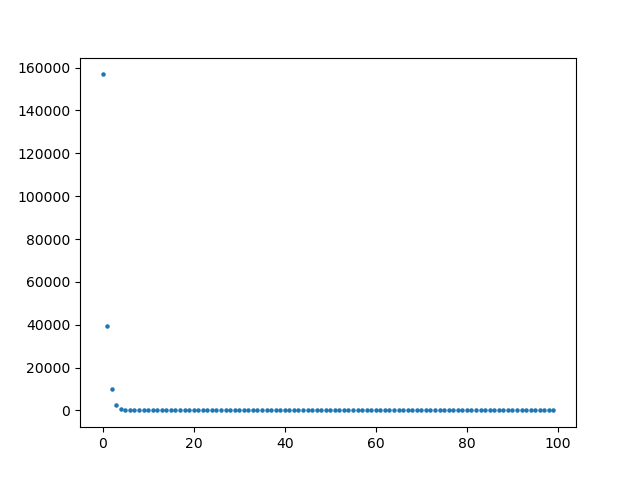
\includegraphics[scale = 0.6]{figures/ADMM_lam=0.1.png}
    \caption{lambda = 0.1}
    \end{figure}


\end{document}
